\documentclass[11pt,a4paper]{article}

\usepackage[margin=2.2cm]{geometry}
\usepackage{amsmath,amssymb,amsthm}
\usepackage{booktabs}
\usepackage{array}
\usepackage{tabularx}
\usepackage[shortlabels]{enumitem}
\usepackage{xcolor}
\usepackage{tikz}
\usepackage{fancyhdr}
\usepackage{setspace}
\usepackage{microtype}
\usepackage{titlesec}
\usepackage{hyperref}
\usepackage{listings}
\usepackage[skins,breakable]{tcolorbox}

\usetikzlibrary{positioning,arrows.meta,calc,fit,shapes.geometric,matrix,decorations.pathreplacing}

\definecolor{ink}{HTML}{222222}
\definecolor{rulegray}{HTML}{444444}
\definecolor{boxline}{HTML}{666666}
\definecolor{boxfill}{HTML}{F4F4F4}
\definecolor{boxtitle}{HTML}{E8E8E8}
\definecolor{g1}{HTML}{D0D0D0}
\definecolor{g2}{HTML}{9A9A9A}
\definecolor{g3}{HTML}{5A5A5A}

\hypersetup{
  colorlinks=true,
  linkcolor=black,
  urlcolor=black,
  pdftitle={MTL 458 Lecture 22A: Persistence: RAID},
  pdfauthor={Minati De, IIT Delhi}
}

\setstretch{1.12}
\raggedbottom
\setlist[itemize]{leftmargin=1.3em,itemsep=0.28em,topsep=0.35em}
\setlist[enumerate]{leftmargin=1.5em,itemsep=0.35em,topsep=0.4em}

\titleformat{\section}
  {\Large\bfseries\color{ink}}{\thesection.}{0.6em}{}
  [{\color{rulegray}\titlerule[0.5pt]}]
\titleformat{\subsection}
  {\large\bfseries\color{ink}}{\thesubsection}{0.55em}{}
\titleformat{\subsubsection}
  {\normalsize\bfseries\color{ink}}{\thesubsubsection}{0.5em}{}

\titlespacing*{\section}{0pt}{1.35em}{0.7em}
\titlespacing*{\subsection}{0pt}{1.05em}{0.45em}

\pagestyle{fancy}
\fancyhf{}
\renewcommand{\headrulewidth}{0.4pt}
\renewcommand{\footrulewidth}{0.3pt}
\fancyhead[L]{\small\color{ink}MTL 458 \textbullet\ Operating Systems}
\fancyhead[R]{\small\color{ink}Lecture 22A: Persistence: RAID}
\fancyfoot[C]{\small\thepage}
\setlength{\headheight}{14pt}

% ---------------------------------------------------------------------------
% Boxes
% ---------------------------------------------------------------------------
\tcbset{
  commonbox/.style={
    colback=boxfill, colframe=boxline, boxrule=0.5pt,
    left=6pt, right=6pt, top=5pt, bottom=5pt,
    fonttitle=\bfseries, coltitle=black, colbacktitle=boxtitle,
    enhanced, sharp corners=south, breakable
  }
}
\newtcolorbox{keybox}[1][]{commonbox, title={#1}}
\newtcolorbox{quizbox}[1][]{commonbox, title={#1}}
\newtcolorbox{solbox}[1][]{commonbox, title={#1}}
\newtcolorbox{warnbox}[1][]{commonbox, title={#1}}
\newtcolorbox{defbox}[1][]{commonbox, title={#1}}

% Start a new page unless at least #1 of vertical space remains
\makeatletter
\newcommand{\keepspace}[1]{\par\penalty-100\begingroup
  \setlength{\dimen@}{#1}\dimen@ii\pagegoal\advance\dimen@ii-\pagetotal
  \ifdim\dimen@>\dimen@ii\ifdim\dimen@ii>\z@\vfil\fi\break\fi\endgroup}
\makeatother

% ---------------------------------------------------------------------------
% Disk-array grids.
% \blockgrid{headers}{rows}{extra tikz}
%   headers: comma list (one per disk); rows: {{..},{..},...}, one list per
%   offset. A cell whose value is P is drawn dark (parity).
%   Cells are named c-<row>-<col> (both from 0).
% ---------------------------------------------------------------------------
\tikzset{
  cell/.style={draw=boxline, fill=g1, minimum width=1.15cm, minimum height=0.5cm,
               inner sep=0pt, font=\small},
  pcell/.style={cell, fill=g3, text=white, font=\small\bfseries},
  stripebox/.style={draw=black, very thick, rounded corners=2pt},
}
\def\Pmark{P}
\newcommand{\blockgrid}[3]{%
\begin{tikzpicture}[x=1.45cm,y=0.5cm]
  \foreach \h [count=\c from 0] in {#1}
    \node[font=\small\bfseries, anchor=south] at (\c,0.55) {\h};
  \foreach \row [count=\r from 0] in {#2}
    \foreach \v [count=\c from 0] in \row {%
      \ifx\v\Pmark \node[pcell] (c-\r-\c) at (\c,-\r) {P};%
      \else \node[cell] (c-\r-\c) at (\c,-\r) {\v};\fi}
  #3
\end{tikzpicture}}

% Mirrored pair of disks with 4 offsets (crash example).
% \crashpanel{disk0 values}{disk1 values}{extra tikz}
\tikzset{ccell/.style={draw=boxline, fill=g1, minimum width=0.6cm, minimum height=0.45cm,
                       inner sep=0pt, font=\small\bfseries},
         newcell/.style={ccell, fill=g3, text=white}}
\newcommand{\crashpanel}[3]{%
\begin{tikzpicture}[x=0.7cm,y=0.45cm]
  \node[font=\scriptsize\bfseries] at (0,1.1) {Disk 0};
  \node[font=\scriptsize\bfseries] at (1.75,1.1) {Disk 1};
  \foreach \v [count=\r from 0] in {#1} \node[ccell] at (0,-\r) {\v};
  \foreach \v [count=\r from 0] in {#2} \node[ccell] at (1.75,-\r) {\v};
  \foreach \r in {0,...,3} \node[font=\scriptsize, text=g3] at (-0.85,-\r) {\r};
  \path (-1.1,0) -- (4.4,0);
  #3
\end{tikzpicture}}

\begin{document}

% ===========================================================================
% Title
% ===========================================================================
\begin{center}
{\small\itshape Made by Arpit's Milo}\\[0.3em]
{\color{rulegray}\rule{\textwidth}{1.1pt}}\\[0.45em]
{\LARGE\bfseries Operating Systems}\\[0.25em]
{\Large\bfseries MTL 458 \textperiodcentered\ Lecture 22A}\\[0.35em]
{\LARGE\bfseries Persistence: RAID}\\[0.35em]
{\large Minati De}\\[0.15em]
{\normalsize Department of Mathematics, Indian Institute of Technology Delhi}\\[0.35em]
{\color{rulegray}\rule{\textwidth}{1.1pt}}
\end{center}

\vspace{0.4em}
\begin{keybox}[Questions answered in this lecture]
\begin{itemize}
  \item Why more than one disk?
  \item What are the different RAID levels? (\textbf{striping},
        \textbf{mirroring}, \textbf{parity})
  \item Which RAID levels are best for \textbf{reliability}? For
        \textbf{capacity}?
  \item Which are best for \textbf{performance}? (sequential vs.\ random
        reads and writes)
\end{itemize}
\end{keybox}

\tableofcontents
\vspace{0.6em}
\noindent{\color{rulegray}\rule{\textwidth}{0.4pt}}

% ===========================================================================
\section{Why more than one disk?}
% ===========================================================================

\subsection{Only one disk?}

\begin{quizbox}[Sometimes we want many disks --- why?]
\begin{itemize}
  \item \textbf{Capacity} (one disk may be too small);
  \item \textbf{Reliability} (survive a disk failure);
  \item \textbf{Performance} (disks work in parallel).
\end{itemize}
\end{quizbox}

\textbf{Challenge:} most file systems work on only one disk.

\subsection{Solution 1: JBOD and Solution 2: RAID}

\begin{center}
\begin{minipage}[t]{0.46\textwidth}\centering
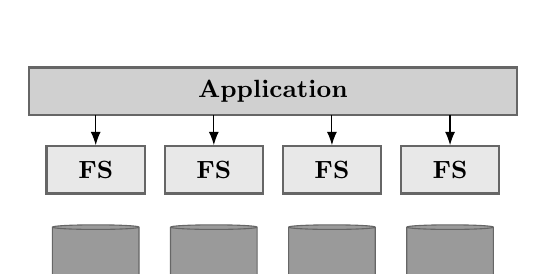
\begin{tikzpicture}[
    lay/.style={draw=boxline, thick, minimum height=0.6cm, font=\small\bfseries},
    cyl/.style={cylinder, shape border rotate=90, aspect=0.25, draw=boxline,
                fill=g2, minimum width=1.1cm, minimum height=0.75cm}]
  \node[lay, fill=g1, minimum width=6.2cm] at (2.25,2.2) {Application};
  \foreach \i in {0,...,3} {
    \node[lay, fill=boxtitle, minimum width=1.25cm] (fs\i) at (1.5*\i,1.2) {FS};
    \node[cyl] at (1.5*\i,0.1) {};
    \draw[-{Latex}] (1.5*\i,1.9) -- (fs\i.north);
  }
\end{tikzpicture}\\[0.3em]
{\small (a) \textbf{JBOD}: \textbf{J}ust a \textbf{B}unch \textbf{O}f
\textbf{D}isks. The application is smart and stores different files on
different file systems, one per disk.}
\end{minipage}\hfill
\begin{minipage}[t]{0.46\textwidth}\centering
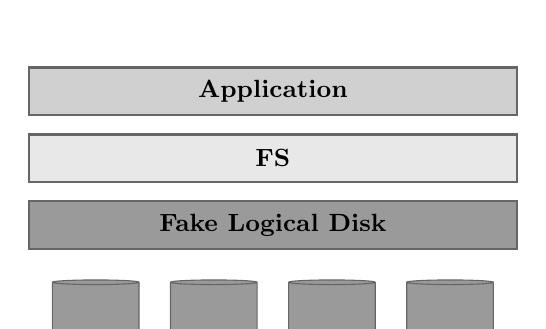
\begin{tikzpicture}[
    lay/.style={draw=boxline, thick, minimum height=0.6cm, font=\small\bfseries},
    cyl/.style={cylinder, shape border rotate=90, aspect=0.25, draw=boxline,
                fill=g2, minimum width=1.1cm, minimum height=0.75cm}]
  \node[lay, fill=g1, minimum width=6.2cm] at (2.25,2.9) {Application};
  \node[lay, fill=boxtitle, minimum width=6.2cm] at (2.25,2.05) {FS};
  \node[lay, fill=g2, minimum width=6.2cm] at (2.25,1.2) {Fake Logical Disk};
  \foreach \i in {0,...,3} \node[cyl] at (1.5*\i,0.1) {};
\end{tikzpicture}\\[0.3em]
{\small (b) \textbf{RAID}: \textbf{R}edundant \textbf{A}rray of
\textbf{I}nexpensive \textbf{D}isks. Build one logical disk from many
physical disks; a single FS sits on top of it.}
\end{minipage}
\end{center}


\begin{center}
\renewcommand{\arraystretch}{1.2}
\begin{tabularx}{0.92\textwidth}{@{}X X@{}}
\toprule
\textbf{RAID is:} & \textbf{The logical disk gives:} \\
\midrule
\textbf{transparent} (looks like one disk) & \textbf{capacity} \\
\textbf{deployable} (no FS changes needed) & \textbf{performance} \\
 & \textbf{reliability} \\
\bottomrule
\end{tabularx}
\end{center}

\subsection{Why inexpensive disks?}

\begin{itemize}
  \item \textbf{Economies of scale!} Commodity disks cost less.
  \item We can buy many commodity hardware components for the same price as
        a few high-end components.
  \item \textbf{Strategy:} write software to build \textbf{high-quality
        logical devices from many cheap devices}.
  \item \textbf{Alternative to RAID:} buy an expensive, high-end disk.
\end{itemize}

\keepspace{9\baselineskip}
% ===========================================================================
\section{General strategies: mapping and redundancy}
% ===========================================================================


\keepspace{9\baselineskip}
\subsection{Mapping: build a fast, large disk from smaller ones}

\begin{center}
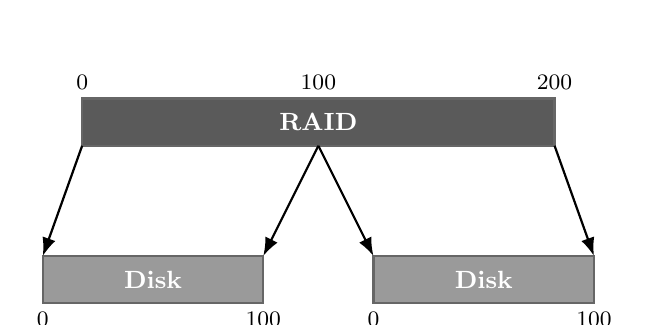
\begin{tikzpicture}[
    disk/.style={draw=boxline, thick, fill=g2, minimum width=2.8cm, minimum height=0.6cm,
                 font=\small\bfseries, text=white}]
  \node[draw=boxline, thick, fill=g3, minimum width=6cm, minimum height=0.6cm,
        font=\small\bfseries, text=white] at (3,2) {RAID};
  \foreach \x/\l in {0/0,3/100,6/200} \node[font=\footnotesize] at (\x,2.5) {\l};
  \node[disk] at (0.9,0) {Disk};
  \node[disk] at (5.1,0) {Disk};
  \foreach \x/\l in {-0.5/0,2.3/100,3.7/0,6.5/100} \node[font=\footnotesize] at (\x,-0.5) {\l};
  \draw[-{Latex}, thick] (0,1.7) -- (-0.5,0.3);
  \draw[-{Latex}, thick] (3,1.7) -- (2.3,0.3);
  \draw[-{Latex}, thick] (3,1.7) -- (3.7,0.3);
  \draw[-{Latex}, thick] (6,1.7) -- (6.5,0.3);
\end{tikzpicture}
\end{center}

Two 100-block disks form one 200-block logical disk (logical 0--99 on the
left disk, 100--199 on the right).

\keepspace{9\baselineskip}
\subsection{Redundancy: add even more disks for reliability}

\begin{center}
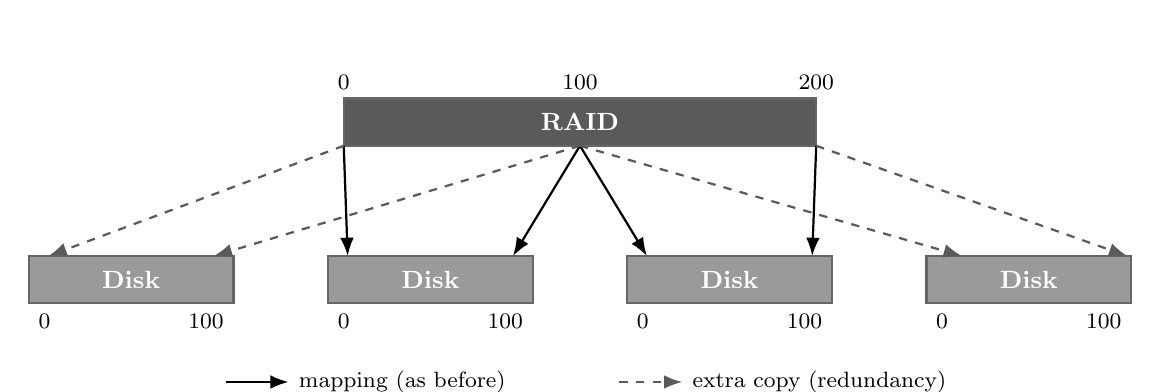
\begin{tikzpicture}[
    disk/.style={draw=boxline, thick, fill=g2, minimum width=2.6cm, minimum height=0.6cm,
                 font=\small\bfseries, text=white}]
  \node[draw=boxline, thick, fill=g3, minimum width=6cm, minimum height=0.6cm,
        font=\small\bfseries, text=white] at (3,2) {RAID};
  \foreach \x/\l in {0/0,3/100,6/200} \node[font=\footnotesize] at (\x,2.5) {\l};
  \foreach \c in {-2.7,1.1,4.9,8.7} {
    \node[disk] at (\c,0) {Disk};
    \node[font=\footnotesize, anchor=north west] at (\c-1.3,-0.32) {0};
    \node[font=\footnotesize, anchor=north east] at (\c+1.3,-0.32) {100};
  }
  % original mapping (solid)
  \draw[-{Latex}, thick] (0,1.7) -- (0.05,0.3);
  \draw[-{Latex}, thick] (3,1.7) -- (2.15,0.3);
  \draw[-{Latex}, thick] (3,1.7) -- (3.85,0.3);
  \draw[-{Latex}, thick] (6,1.7) -- (5.95,0.3);
  % redundant copies (dashed)
  \draw[-{Latex}, thick, dashed, g3] (0,1.7) -- (-3.75,0.3);
  \draw[-{Latex}, thick, dashed, g3] (3,1.7) -- (-1.65,0.3);
  \draw[-{Latex}, thick, dashed, g3] (3,1.7) -- (7.85,0.3);
  \draw[-{Latex}, thick, dashed, g3] (6,1.7) -- (9.95,0.3);
  % legend
  \draw[-{Latex}, thick] (-1.5,-1.3) -- (-0.7,-1.3) node[right, font=\footnotesize] {mapping (as before)};
  \draw[-{Latex}, thick, dashed, g3] (3.5,-1.3) -- (4.3,-1.3) node[right, font=\footnotesize, text=black] {extra copy (redundancy)};
\end{tikzpicture}
\end{center}

The two inner disks hold the mapping; the two outer disks hold extra
copies, so every block survives one disk failure.

\subsection{Mapping}

\textbf{How should we map logical block addresses to physical block
addresses?} Some similarity to virtual memory:
\begin{enumerate}
  \item \textbf{Dynamic} mapping: use a data structure (hash table, tree).
        Example: \textbf{page tables}.
  \item \textbf{Static} mapping: use simple math. Example: \textbf{RAID}.
\end{enumerate}

\subsection{Redundancy}

There are \textbf{trade-offs} to the amount of redundancy:
\begin{itemize}
  \item \textbf{Increase} the number of copies: improves
        \textbf{reliability} (and maybe \textbf{performance}).
  \item \textbf{Decrease} the number of copies (\textbf{deduplication}):
        improves \textbf{space efficiency}.
\end{itemize}

\keepspace{9\baselineskip}
% ===========================================================================
\section{Reasoning about RAID}
% ===========================================================================

\begin{defbox}[Three things to reason about]
\begin{itemize}
  \item \textbf{RAID:} a system for mapping logical to physical blocks.
  \item \textbf{Workload:} the types of reads/writes issued by applications
        (sequential vs.\ random).
  \item \textbf{Metric:} capacity, reliability, performance.
\end{itemize}
\end{defbox}

\subsection{RAID decisions}

\begin{itemize}
  \item Which logical blocks map to which physical blocks?
  \item How do we use extra physical blocks (if any)?
\end{itemize}
Different \textbf{RAID levels} make different trade-offs in answering these
two questions.

\subsection{Workloads}

\begin{center}
\begin{minipage}[t]{0.4\textwidth}
\textbf{Reads}
\begin{itemize}
  \item One operation
  \item Steady-state I/O
  \begin{itemize}
    \item Sequential
    \item Random
  \end{itemize}
\end{itemize}
\end{minipage}\hspace{2em}
\begin{minipage}[t]{0.4\textwidth}
\textbf{Writes}
\begin{itemize}
  \item One operation
  \item Steady-state I/O
  \begin{itemize}
    \item Sequential
    \item Random
  \end{itemize}
\end{itemize}
\end{minipage}
\end{center}

(One operation is measured by latency; steady-state I/O by throughput.)

\keepspace{9\baselineskip}
\subsection{Metrics}

\begin{defbox}[Metrics and notation]
\begin{itemize}
  \item \textbf{Capacity:} how much space can apps use?
  \item \textbf{Reliability:} how many disks can we safely lose?
        (\textbf{assume fail stop!})
  \item \textbf{Performance:} how long does each workload take?
\end{itemize}
Normalize each to the characteristics of one disk:
\[
\begin{array}{r@{\;:=\;}l}
  N & \text{number of disks} \\
  C & \text{capacity of 1 disk} \\
  S & \text{sequential throughput of 1 disk} \\
  R & \text{random throughput of 1 disk} \\
  D & \text{latency of one small I/O operation}
\end{array}
\]
\end{defbox}

\keepspace{9\baselineskip}
% ===========================================================================
\section{RAID-0: Striping}
% ===========================================================================

\textbf{Optimize for capacity. No redundancy.}

\keepspace{9\baselineskip}
\subsection{Two disks}

\begin{center}
\begin{minipage}{0.66\textwidth}\centering
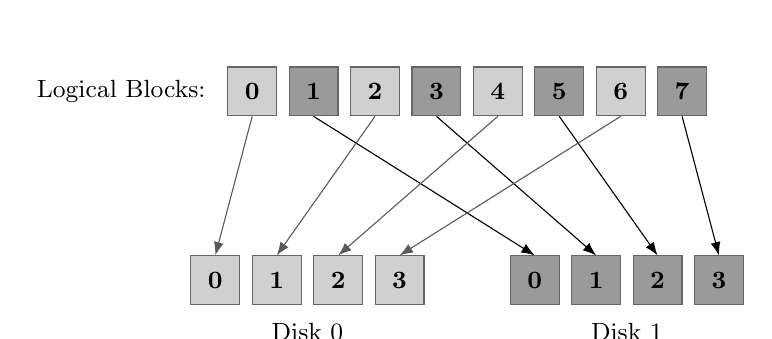
\begin{tikzpicture}[x=0.78cm,
    lb/.style={draw=boxline, minimum size=0.62cm, inner sep=0pt, font=\small\bfseries}]
  \node[font=\small, anchor=east] at (-0.6,2.4) {Logical Blocks:};
  \foreach \i in {0,...,7} {
    \pgfmathtruncatemacro{\odd}{mod(\i,2)}
    \ifnum\odd=0 \node[lb, fill=g1] (L\i) at (\i,2.4) {\i};
    \else \node[lb, fill=g2] (L\i) at (\i,2.4) {\i};\fi
  }
  \foreach \i in {0,...,3} {
    \node[lb, fill=g1] (A\i) at (\i-0.6,0) {\i};
    \node[lb, fill=g2] (B\i) at (\i+4.6,0) {\i};
  }
  \node[font=\small] at (0.9,-0.65) {Disk 0};
  \node[font=\small] at (6.1,-0.65) {Disk 1};
  \foreach \i in {0,...,3} {
    \pgfmathtruncatemacro{\e}{2*\i}
    \pgfmathtruncatemacro{\o}{2*\i+1}
    \draw[-{Latex}, g3] (L\e.south) -- (A\i.north);
    \draw[-{Latex}, black] (L\o.south) -- (B\i.north);
  }
\end{tikzpicture}
\end{minipage}\hfill
\begin{minipage}{0.28\textwidth}\centering
\renewcommand{\arraystretch}{1.15}
\begin{tabular}{cc}
\toprule
\textbf{Disk 0} & \textbf{Disk 1} \\
\midrule
0 & 1 \\ 2 & 3 \\ 4 & 5 \\ 6 & 7 \\
\bottomrule
\end{tabular}
\end{minipage}
\end{center}

Disk boxes show physical offsets; the table shows which logical block is at
each offset (even blocks on Disk 0, odd on Disk 1).

\keepspace{9\baselineskip}
\subsection{Four disks, stripes and the mapping formula}

\begin{center}
\blockgrid{Disk 0,Disk 1,Disk 2,Disk 3}
  {{0,1,2,3},{4,5,6,7},{8,9,10,11},{12,13,14,15}}
  {\draw[stripebox] ($(c-0-0.north west)+(-0.1,0.08)$) rectangle ($(c-0-3.south east)+(0.1,-0.08)$);
   \node[anchor=east, font=\small\bfseries] at ($(c-0-0.west)+(-0.2,0)$) {stripe:};
   \foreach \r in {0,...,3} \node[font=\scriptsize, text=g3] at ($(c-\r-3.east)+(0.45,0)$) {off \r};}
\end{center}

\begin{defbox}[Stripe]
A \textbf{stripe} is one row: the blocks at the same offset on every disk
(here 0, 1, 2, 3).
\end{defbox}

\keepspace{9\baselineskip}
\begin{quizbox}[Given logical address \(A\), find Disk and Offset]
With chunk size 1 (integer division):
\[
  \text{Disk} = A \bmod \text{disk\_count}, \qquad
  \text{Offset} = A \,/\, \text{disk\_count}.
\]
E.g.\ \(A = 6\): Disk 2, offset 1.
\end{quizbox}

{\small (The slides label the fourth disk ``Disk 4'' in all the 4-disk
tables of this lecture; it is the fourth disk of disks \(0..3\), so it should
be ``Disk 3'', as drawn here.)}

\keepspace{9\baselineskip}
\subsection{Chunk size}

The \textbf{chunk size} is how many consecutive logical blocks are placed on
one disk before moving to the next disk.

\begin{center}
\begin{minipage}[t]{0.48\textwidth}\centering
\blockgrid{Disk 0,Disk 1,Disk 2,Disk 3}
  {{0,1,2,3},{4,5,6,7},{8,9,10,11},{12,13,14,15}}
  {\draw[stripebox] ($(c-0-0.north west)+(-0.1,0.08)$) rectangle ($(c-0-3.south east)+(0.1,-0.08)$);}\\[0.3em]
{\small (a) Chunk size \(=1\). A stripe is one row.}
\end{minipage}\hfill
\begin{minipage}[t]{0.48\textwidth}\centering
\blockgrid{Disk 0,Disk 1,Disk 2,Disk 3}
  {{0,2,4,6},{1,3,5,7},{8,10,12,14},{9,11,13,15}}
  {\foreach \c in {0,...,3} {
     \draw[thick, rounded corners=4pt] ($(c-0-\c.north west)+(0.06,-0.05)$) rectangle ($(c-1-\c.south east)+(-0.06,0.05)$);
     \draw[thick, rounded corners=4pt] ($(c-2-\c.north west)+(0.06,-0.05)$) rectangle ($(c-3-\c.south east)+(-0.06,0.05)$);}
   \draw[stripebox] ($(c-0-0.north west)+(-0.1,0.08)$) rectangle ($(c-1-3.south east)+(0.1,-0.08)$);}\\[0.3em]
{\small (b) Chunk size \(=2\). Each rounded box is a chunk; a stripe (outer
box) is two rows.}
\end{minipage}
\end{center}

With chunk size 2, blocks 0--1 are a chunk on Disk 0, 2--3 on Disk 1, and so
on. \textbf{For the rest of the lecture, assume a chunk size of 1.}
{\small (On the slide, the ``stripe'' box in table (b) is drawn around the
rows 1,3,5,7 and 8,10,12,14, which straddles two stripes. A stripe is one
chunk from every disk, so it is blocks 0--7 (rows 0--1) as drawn here, or
8--15.)}

\keepspace{9\baselineskip}
\subsection{RAID-0: analysis}

\begin{quizbox}[RAID-0: capacity, failures, latency, throughput]
\begin{itemize}
  \item \textbf{What is capacity?}\quad \textbf{\(N \cdot C\).}\enspace Every block holds user data; nothing is spent on redundancy.
  \item \textbf{How many disks can fail?}\quad \textbf{\(0\).}\enspace Losing any disk loses every block on it (and so pieces of almost every large file).
  \item \textbf{Latency?}\quad \textbf{\(D\).}\enspace A single small request goes to exactly one disk, so it takes as long as on one disk.
  \item \textbf{Throughput (seq., random)?}\quad \textbf{\(N\cdot S\), \(N \cdot R\).}\enspace All \(N\) disks work in parallel on a large stream or on many random requests.
\end{itemize}
\end{quizbox}

\begin{keybox}[Takeaway]
\textbf{Buying more disks improves throughput, but not latency!}
\end{keybox}

\keepspace{9\baselineskip}
% ===========================================================================
\section{RAID-1: Mirroring}
% ===========================================================================

\textbf{Keep two copies of all data.}

\begin{center}
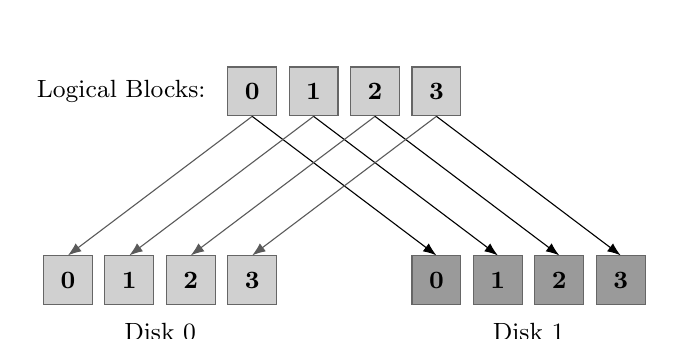
\begin{tikzpicture}[x=0.78cm,
    lb/.style={draw=boxline, minimum size=0.62cm, inner sep=0pt, font=\small\bfseries}]
  \node[font=\small, anchor=east] at (1.4,2.4) {Logical Blocks:};
  \foreach \i in {0,...,3} \node[lb, fill=g1] (L\i) at (\i+2,2.4) {\i};
  \foreach \i in {0,...,3} {
    \node[lb, fill=g1] (A\i) at (\i-1,0) {\i};
    \node[lb, fill=g2] (B\i) at (\i+5,0) {\i};
    \draw[-{Latex}, g3] (L\i.south) -- (A\i.north);
    \draw[-{Latex}] (L\i.south) -- (B\i.north);
  }
  \node[font=\small] at (0.5,-0.65) {Disk 0};
  \node[font=\small] at (6.5,-0.65) {Disk 1};
\end{tikzpicture}
\end{center}


\keepspace{9\baselineskip}
\subsection{RAID-1 layout}

\begin{center}
\begin{minipage}[t]{0.3\textwidth}\centering
\blockgrid{Disk 0,Disk 1}{{0,0},{1,1},{2,2},{3,3}}{}\\[0.3em]
{\small (a) 2 disks}
\end{minipage}\hfill
\begin{minipage}[t]{0.62\textwidth}\centering
\blockgrid{Disk 0,Disk 1,Disk 2,Disk 3}{{0,0,1,1},{2,2,3,3},{4,4,5,5},{6,6,7,7}}
  {\draw[decorate, decoration={brace, mirror, amplitude=4pt}, thick]
     ($(c-3-0.south west)+(0,-0.12)$) -- ($(c-3-1.south east)+(0,-0.12)$)
     node[midway, below=4pt, font=\scriptsize] {mirror pair};
   \draw[decorate, decoration={brace, mirror, amplitude=4pt}, thick]
     ($(c-3-2.south west)+(0,-0.12)$) -- ($(c-3-3.south east)+(0,-0.12)$)
     node[midway, below=4pt, font=\scriptsize] {mirror pair};}\\[0.3em]
{\small (b) 4 disks}
\end{minipage}
\end{center}

\begin{itemize}
  \item With \textbf{2 disks}, Disk 1 is a block-for-block copy of Disk 0.
  \item With \textbf{4 disks}, two mirrored pairs: (Disk 0, Disk 1) holds the
        even blocks, (Disk 2, Disk 3) the odd blocks.
\end{itemize}
{\small (Slides label the fourth disk ``Disk 4''; it should be Disk 3.)}

\keepspace{9\baselineskip}
\subsection{RAID-1 with 4 disks: how many disks can fail?}

\begin{defbox}[Fail-stop disks]
Assume disks are \textbf{fail-stop}:
\begin{itemize}
  \item each disk works or it doesn't;
  \item the system knows when a disk fails.
\end{itemize}
\textbf{Tougher errors} (not covered by this model):
\begin{itemize}
  \item \textbf{latent sector errors}: the disk works but some sector can no
        longer be read;
  \item \textbf{silent data corruption}: the disk returns wrong data without
        reporting any error.
\end{itemize}
\end{defbox}

\keepspace{9\baselineskip}
\begin{quizbox}[How many disks can fail?]
\textbf{1 for sure (or maybe \(N/2\))}: up to \(N/2\) if each failed disk is
in a different mirror pair (e.g.\ Disks 0 and 2), but losing both disks of
one pair loses data.
\end{quizbox}

\keepspace{9\baselineskip}
\subsection{RAID-1: analysis}

\begin{quizbox}[RAID-1: capacity, failures, latency]
\begin{itemize}
  \item \textbf{What is capacity?}\quad \textbf{\(N/2 \cdot C\).}\enspace Every block is stored twice.
  \item \textbf{How many disks can fail?}\quad \textbf{\(1\) (or maybe \(N/2\)).}\enspace See above.
  \item \textbf{Latency (read, write)?}\quad \textbf{\(D\), \(D\).}\enspace A read goes to one copy. A write goes to both copies in parallel, so it also takes \(D\).
\end{itemize}
\end{quizbox}

\keepspace{9\baselineskip}
\subsection{RAID-1: throughput}

\begin{quizbox}[What is the steady-state throughput for each workload?]
\begin{itemize}
  \item \textbf{Random reads}\quad \textbf{\(N \cdot R\).}\enspace Each read can go to either copy, so reads are spread over all \(N\) disks. This is the best case for mirroring.
  \item \textbf{Random writes}\quad \textbf{\(N/2 \cdot R\).}\enspace Each logical write becomes two physical writes. All disks are busy, but only half of the work is ``useful''.
  \item \textbf{Sequential writes}\quad \textbf{\(N/2 \cdot S\).}\enspace Same reason: every block is written twice, so only half the bandwidth delivers new data.
  \item \textbf{Sequential reads}\quad \textbf{\(N/2 \cdot S\).}\enspace \textbf{Book: \(N/2\cdot S\) (other models: \(N \cdot S\)).}
\end{itemize}
\end{quizbox}

\textbf{Why only \(N/2 \cdot S\) for sequential reads (book)?} When alternating
copies, each disk skips every other block, and while it rotates over a
skipped block it delivers no data, so each disk gives half its bandwidth.

\keepspace{9\baselineskip}
% ===========================================================================
\section{Crashes: the consistent-update problem}
% ===========================================================================

A mirrored write must update \emph{two} disks. What if the machine crashes
in between? (Dark cells were just changed.)

\begin{center}
\begin{minipage}[t]{0.245\textwidth}\centering
\crashpanel{A,B,C,D}{A,B,C,D}{}\\
{\footnotesize (1) Initial state: both copies hold A, B, C, D.}
\end{minipage}\hfill
\begin{minipage}[t]{0.245\textwidth}\centering
\crashpanel{A,B,C,D}{A,B,C,D}{}\\
{\footnotesize (2) \texttt{write(A) to 2} is issued; nothing changed yet.}
\end{minipage}\hfill
\begin{minipage}[t]{0.245\textwidth}\centering
\crashpanel{A,B,A,D}{A,B,C,D}{\node[newcell] at (0,-2) {A};}\\
{\footnotesize (3) Disk 0 updated (C\(\to\)A); Disk 1 still has C. The
copies disagree for now.}
\end{minipage}\hfill
\begin{minipage}[t]{0.245\textwidth}\centering
\crashpanel{A,B,A,D}{A,B,A,D}{\node[newcell] at (1.75,-2) {A};}\\
{\footnotesize (4) Disk 1 updated too: the write completed and the copies
agree again.}
\end{minipage}

\vspace{0.8em}
\begin{minipage}[t]{0.245\textwidth}\centering
\crashpanel{A,B,A,D}{A,B,A,D}{}\\
{\footnotesize (5) \texttt{write(T) to 3} is issued.}
\end{minipage}\hfill
\begin{minipage}[t]{0.245\textwidth}\centering
\crashpanel{A,B,A,D}{A,B,A,T}{\node[newcell] at (1.75,-3) {T};}\\
{\footnotesize (6) Disk 1 updated (D\(\to\)T); Disk 0 still has D.}
\end{minipage}\hfill
\begin{minipage}[t]{0.245\textwidth}\centering
\crashpanel{A,B,A,D}{A,B,A,T}{\node[font=\scriptsize\bfseries, rotate=-12] at (3.45,-1.5) {CRASH!!!};}\\
{\footnotesize (7) The machine crashes before Disk 0 is updated.}
\end{minipage}\hfill
\begin{minipage}[t]{0.245\textwidth}\centering
\crashpanel{A,B,A,D}{A,B,A,T}{\draw[line width=1.6pt] (-0.43,-3.5) rectangle (0.43,-2.5);
  \draw[line width=1.6pt] (1.32,-3.5) rectangle (2.18,-2.5);
  \node[font=\small] at (0.875,-3) {\(\neq\)};
  \node[font=\Large\bfseries] at (2.75,-3) {?};}\\
{\footnotesize (8) After reboot, how to tell which data is right?}
\end{minipage}
\end{center}

\keepspace{9\baselineskip}
\begin{quizbox}[After reboot, how to tell which data is right?]
From the disks alone, \textbf{we cannot}: D and T both look valid. The
update should be \textbf{atomic}, so the RAID must record the pending write
before doing it (and finish it after the crash).
\end{quizbox}

\subsection{H/W solution}

\begin{keybox}[Consistent-update problem]
\begin{itemize}
  \item \textbf{Problem:} the \textbf{consistent-update problem}.
  \item Use \textbf{non-volatile RAM} in the RAID controller (it records the
        pending write and survives the crash).
  \item Software RAID controllers (e.g.\ Linux \texttt{md}) don't have this
        option.
\end{itemize}
\end{keybox}

\keepspace{9\baselineskip}
% ===========================================================================
\section{Capacity vs.\ reliability}
% ===========================================================================

\begin{center}
\begin{minipage}{0.45\textwidth}\centering
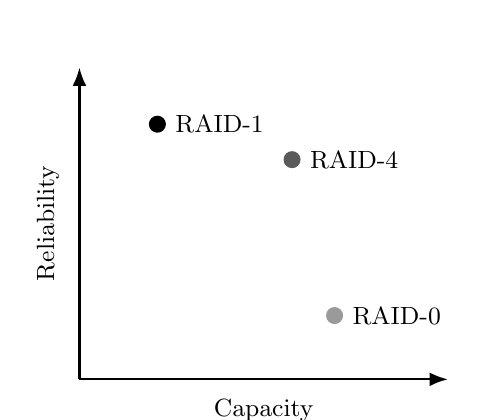
\begin{tikzpicture}[scale=0.9]
  \draw[-{Latex}, thick] (0,0) -- (5.2,0);
  \draw[-{Latex}, thick] (0,0) -- (0,4.4);
  \node[below, font=\small] at (2.6,-0.15) {Capacity};
  \node[rotate=90, above, font=\small] at (-0.15,2.2) {Reliability};
  \fill[black] (1.1,3.6) circle (0.12) node[right=3pt, font=\small] {RAID-1};
  \fill[g3] (3.0,3.1) circle (0.12) node[right=3pt, font=\small, text=black] {RAID-4};
  \fill[g2] (3.6,0.9) circle (0.12) node[right=3pt, font=\small, text=black] {RAID-0};
\end{tikzpicture}
\end{minipage}\hfill
\begin{minipage}{0.5\textwidth}
\begin{itemize}
  \item \textbf{RAID-0}: best capacity, no reliability.
  \item \textbf{RAID-1}: good reliability, half the capacity.
  \item \textbf{RAID-4}: nearly full capacity and tolerates 1 failure.
\end{itemize}
\end{minipage}
\end{center}

\keepspace{12\baselineskip}
% ===========================================================================
\section{RAID-4: Parity}
% ===========================================================================

\begin{keybox}[RAID-4 strategy]
\begin{itemize}
  \item \textbf{Use a parity disk.}
  \item In algebra, if an equation has \(N\) variables and \(N-1\) are known,
        you can often solve for the unknown.
  \item Treat the sectors across disks in a \textbf{stripe} as an equation.
  \item Data on the bad disk is like the \textbf{unknown} in the equation.
\end{itemize}
\end{keybox}

\keepspace{9\baselineskip}
\subsection{Example}

Disk 4 is the \textbf{parity} disk. The slides use \textbf{addition} as the
parity function (parity \(=\) sum of the stripe's data blocks), one row per
slide build:

\begin{center}
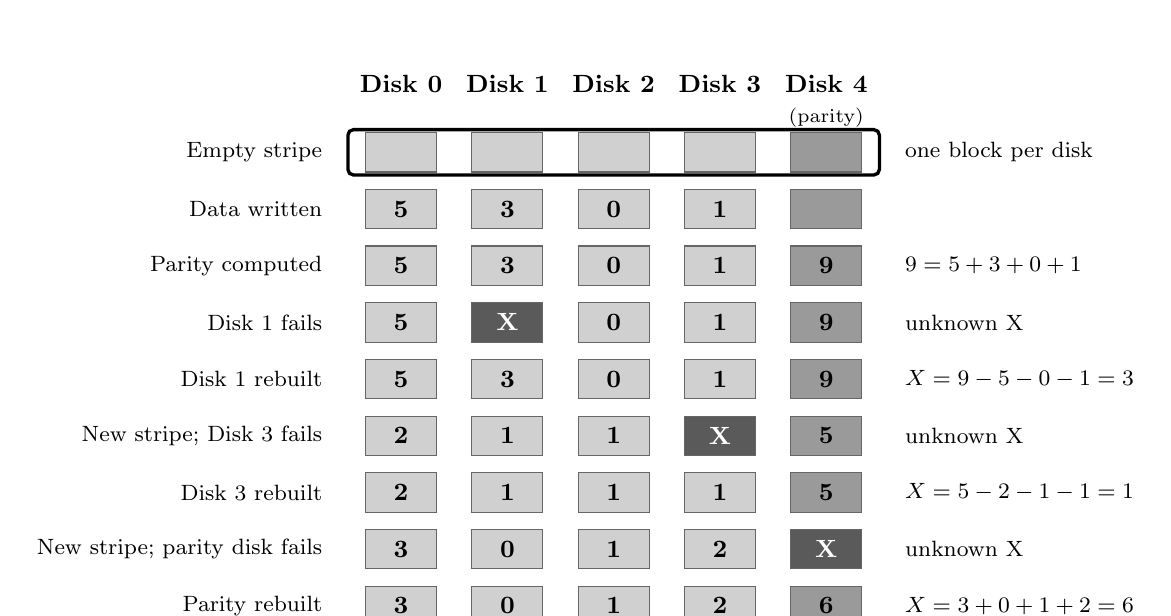
\begin{tikzpicture}[x=1.35cm,y=0.72cm,
    sc/.style={draw=boxline, fill=g1, minimum width=0.9cm, minimum height=0.5cm,
               inner sep=0pt, font=\small\bfseries},
    pc/.style={sc, fill=g2},
    xc/.style={sc, fill=g3, text=white}]
  \foreach \d in {0,...,4} \node[font=\small\bfseries] at (\d,1.2) {Disk \d};
  \node[font=\scriptsize] at (4,0.62) {(parity)};
  % rows: caption, cells (0..3 data, 4 parity), note
  \newcommand{\srow}[8]{%
    \node[anchor=east, font=\footnotesize, align=right] at (-0.65,-#1) {#2};
    \foreach \v [count=\d from 0] in {#3,#4,#5,#6} {
      \ifx\v\Pmark \node[xc] at (\d,-#1) {X};\else \node[sc] at (\d,-#1) {\v};\fi}
    \def\pv{#7}\ifx\pv\Pmark \node[xc] at (4,-#1) {X};\else \node[pc] at (4,-#1) {#7};\fi
    \node[anchor=west, font=\footnotesize] at (4.65,-#1) {#8};}
  \srow{0}{Empty stripe}{}{}{}{}{}{one block per disk}
  \srow{1}{Data written}{5}{3}{0}{1}{}{}
  \srow{2}{Parity computed}{5}{3}{0}{1}{9}{\(9 = 5+3+0+1\)}
  \srow{3}{Disk 1 fails}{5}{P}{0}{1}{9}{unknown X}
  \srow{4}{Disk 1 rebuilt}{5}{3}{0}{1}{9}{\(X = 9-5-0-1 = 3\)}
  \srow{5}{New stripe; Disk 3 fails}{2}{1}{1}{P}{5}{unknown X}
  \srow{6}{Disk 3 rebuilt}{2}{1}{1}{1}{5}{\(X = 5-2-1-1 = 1\)}
  \srow{7}{New stripe; parity disk fails}{3}{0}{1}{2}{P}{unknown X}
  \srow{8}{Parity rebuilt}{3}{0}{1}{2}{6}{\(X = 3+0+1+2 = 6\)}
  \draw[stripebox] (-0.5,-0.4) rectangle (4.5,0.4);
\end{tikzpicture}
\end{center}

With one lost block there is one unknown, so it can always be solved for.

\keepspace{9\baselineskip}
\begin{quizbox}[Which functions are used to compute parity?]
The slides use addition; real RAIDs use bitwise \textbf{XOR}:
\[
  P = D_0 \oplus D_1 \oplus D_2 \oplus D_3, \qquad
  D_1 = D_0 \oplus D_2 \oplus D_3 \oplus P .
\]
(A lost block is the XOR of all the surviving blocks.)
\end{quizbox}

\keepspace{9\baselineskip}
\subsection{RAID-4: analysis}

\begin{quizbox}[RAID-4: capacity, failures, latency]
\begin{itemize}
  \item \textbf{What is capacity?}\quad \textbf{\((N-1) \cdot C\).}\enspace One disk out of \(N\) stores parity.
  \item \textbf{How many disks can fail?}\quad \textbf{\(1\).}\enspace One equation solves for one unknown.
  \item \textbf{Latency (read, write)?}\quad \textbf{\(D\), \(2D\).}\enspace A read takes \(D\) (one data disk). Only a write takes \(2D\): read old data and old parity in parallel, then write new data and new parity in parallel.
\end{itemize}
\end{quizbox}

A small write must also update parity: read old data and old parity, then
write new data and new parity (new parity \(=\) old parity \(-\) old data
\(+\) new data). So the parity disk does a read and a write for
\emph{every} write.

\keepspace{9\baselineskip}
\subsection{RAID-4: throughput}

\begin{quizbox}[What is the steady-state throughput for each workload?]
\begin{itemize}
  \item \textbf{Sequential reads}\quad \textbf{\((N-1)\cdot S\).}\enspace All data disks stream; the parity disk holds no data we need.
  \item \textbf{Sequential writes}\quad \textbf{\((N-1)\cdot S\).}\enspace Write whole stripes (parity computed in memory).
  \item \textbf{Random reads}\quad \textbf{\((N-1)\cdot R\).}\enspace Requests are spread over the \(N-1\) data disks only.
  \item \textbf{Random writes}\quad \textbf{\(R/2\).}\enspace \textbf{Read and write the parity disk.} All writes are serialized on the one parity disk, no matter how large \(N\) is.
\end{itemize}
\end{quizbox}

\begin{warnbox}[The parity bottleneck]
\textbf{How to avoid the parity bottleneck?} Spread the parity over all
disks: RAID-5.
\end{warnbox}

\keepspace{9\baselineskip}
% ===========================================================================
\section{RAID-5: Rotating parity}
% ===========================================================================

\keepspace{9\baselineskip}
\begin{center}
\blockgrid{Disk 0,Disk 1,Disk 2,Disk 3,Disk 4}
  {{--,--,--,--,P},{--,--,--,P,--},{--,--,P,--,--}}
  {\node[font=\large\bfseries] at (2,-3.1) {\(\vdots\)};}
\end{center}

\textbf{Rotate parity across different disks} (``--'' = data, P = parity
of that stripe).

\keepspace{9\baselineskip}
\subsection{RAID-5: analysis}

\begin{quizbox}[RAID-5: capacity, failures, latency]
\begin{itemize}
  \item \textbf{What is capacity?}\quad \textbf{\((N-1) \cdot C\).}\enspace Still one parity block per stripe.
  \item \textbf{How many disks can fail?}\quad \textbf{\(1\).}\enspace Still one equation per stripe.
  \item \textbf{Latency (read, write)?}\quad \textbf{\(D\), \(2D\).}\enspace As in RAID-4.
\end{itemize}
\textbf{Same as RAID-4\ldots}
\end{quizbox}

\keepspace{9\baselineskip}
\subsection{RAID-5: throughput}

\begin{center}
\renewcommand{\arraystretch}{1.25}
\begin{tabular}{@{}lll@{}}
\toprule
\textbf{Workload} & \textbf{RAID-4} & \textbf{RAID-5} \\
\midrule
Sequential reads  & \((N-1)\cdot S\) & \((N-1)\cdot S\) \\
Sequential writes & \((N-1)\cdot S\) & \((N-1)\cdot S\) \\
Random reads      & \((N-1)\cdot R\) & \(N \cdot R\) \\
Random writes     & \(R/2\) (read and write parity disk) & \(N\cdot R/4\) \\
\bottomrule
\end{tabular}
\end{center}

\begin{quizbox}[Why these RAID-5 numbers?]
\begin{itemize}
  \item \textbf{Sequential reads and writes} are the same as RAID-4: in each
        stripe, \(N-1\) blocks are data and one is parity.
  \item \textbf{Random reads: \(N \cdot R\).} Every disk now holds data, so
        reads can be spread over all \(N\) disks.
  \item \textbf{Random writes: \(N \cdot R/4\).} Each write still costs 4
        I/Os, but different writes now use different disks in parallel.
\end{itemize}
{\small (Slide 51 writes \(N * R/4\); the comparison tables write the same
quantity as \(N/4 * R\).)}
\end{quizbox}

\keepspace{9\baselineskip}
% ===========================================================================
\section{RAID level comparisons}
% ===========================================================================

\keepspace{9\baselineskip}
\subsection{Reliability and capacity}

\begin{center}
\renewcommand{\arraystretch}{1.25}
\begin{tabular}{@{}lcc@{}}
\toprule
 & \textbf{Reliability} & \textbf{Capacity} \\
\midrule
RAID-0 & 0 & \(C\cdot N\) \\
RAID-1 & 1 & \(C\cdot N/2\) \\
RAID-4 & 1 & \((N-1)\cdot C\) \\
RAID-5 & 1 & \((N-1)\cdot C\) \\
\bottomrule
\end{tabular}
\end{center}
Reliability is the number of disk failures that can be tolerated for sure
(RAID-1 may survive up to \(N/2\) if lucky).

\keepspace{9\baselineskip}
\subsection{Latency}

\begin{center}
\renewcommand{\arraystretch}{1.25}
\begin{tabular}{@{}lcc@{}}
\toprule
 & \textbf{Read Latency} & \textbf{Write Latency} \\
\midrule
RAID-0 & \(D\) & \(D\) \\
RAID-1 & \(D\) & \(D\) \\
RAID-4 & \(D\) & \(2D\) \\
RAID-5 & \(D\) & \(2D\) \\
\bottomrule
\end{tabular}
\end{center}

\keepspace{9\baselineskip}
\subsection{Throughput}

\begin{center}
\renewcommand{\arraystretch}{1.25}
\begin{tabular}{@{}lcccc@{}}
\toprule
 & \textbf{Seq Read} & \textbf{Seq Write} & \textbf{Rand Read} & \textbf{Rand Write} \\
\midrule
RAID-0 & \(N\cdot S\) & \(N\cdot S\) & \(N\cdot R\) & \(N\cdot R\) \\
RAID-1 & \(N/2\cdot S\) & \(N/2\cdot S\) & \(N\cdot R\) & \(N/2\cdot R\) \\
RAID-4 & \((N-1)\cdot S\) & \((N-1)\cdot S\) & \((N-1)\cdot R\) & \(R/2\) \\
RAID-5 & \((N-1)\cdot S\) & \((N-1)\cdot S\) & \(N\cdot R\) & \(N/4\cdot R\) \\
\bottomrule
\end{tabular}
\end{center}

\begin{keybox}[RAID-5 is strictly better than RAID-4]
Same as RAID-4 except better random I/O, so RAID-4 can be dropped.
\end{keybox}

\keepspace{9\baselineskip}
\subsection{Final comparison: RAID-0, RAID-1, RAID-5}

\begin{center}
\renewcommand{\arraystretch}{1.25}
\begin{tabular}{@{}lcccc@{}}
\toprule
 & \textbf{Seq Read} & \textbf{Seq Write} & \textbf{Rand Read} & \textbf{Rand Write} \\
\midrule
RAID-0 & \(N\cdot S\) & \(N\cdot S\) & \(N\cdot R\) & \(N\cdot R\) \\
RAID-1 & \(N/2\cdot S\) & \(N/2\cdot S\) & \(N\cdot R\) & \(N/2\cdot R\) \\
RAID-5 & \((N-1)\cdot S\) & \((N-1)\cdot S\) & \(N\cdot R\) & \(N/4\cdot R\) \\
\bottomrule
\end{tabular}
\end{center}

\begin{keybox}[Takeaways]
\begin{itemize}
  \item \textbf{RAID-0 is always fastest and has the best capacity} (but at
        the cost of reliability): it has the best (or tied-best) throughput
        in every column and capacity \(N\cdot C\), but tolerates 0 failures.
  \item \textbf{RAID-5 is better than RAID-1 for sequential workloads}:
        \((N-1)\cdot S\) vs.\ \(N/2\cdot S\), and \(N-1 > N/2\) for \(N>2\).
  \item \textbf{RAID-1 is better than RAID-5 for random workloads}: random
        reads are equal (\(N\cdot R\)), and random writes are \(N/2\cdot R\)
        vs.\ \(N/4\cdot R\), twice as fast on RAID-1.
\end{itemize}
\end{keybox}

\keepspace{9\baselineskip}
% ===========================================================================
\section{Summary}
% ===========================================================================

\begin{keybox}[Summary]
\begin{itemize}
  \item There are \textbf{many engineering trade-offs} with RAID: capacity,
        reliability, and performance for different workloads.
  \item RAID presents a \textbf{block-based interface}: it is a very
        deployable and popular storage solution because it is
        \textbf{transparent} to the file system and applications.
  \item Mapping in RAID is \textbf{static} (simple math): the RAID-0
        (chunk size 1) mapping is Disk \(= A \bmod N\) and Offset \(= A / N\).
  \item Mirrored and parity RAIDs face the \textbf{consistent-update
        problem} on crashes; hardware RAID solves it with NVRAM.
\end{itemize}
\end{keybox}


\end{document}
